%*******10********20********30********40********50********60********70********80

% For all chapters, use the newdefined chap{} instead of chapter{}
% This will make the text at the top-left of the page be the same as the chapter

\chap{Results: The Malaria Co-authorship Network}
\label{chap:malaria}
%\section{Background}
%Malaria remains one of the three major public health concerns in Sub Saharan Africa where it affects millions of people and impact negatively on their socioeconomic life \cite{davis_emerging_2001}. In the Millenium Declaration, Malaria has been given a special attention in terms of the successful achievement of the $6^{th}$ development goal of the Millenium Challenge \cite{assembly_united_2000}. In the Republic of Benin, initiatives such as the US President's Malaria Initiative have supported governmental and non-governmental organizations to reduce the mortality and morbidity related to Malaria \cite{arthur_institute_2014,stoops_presidents_2008}. With these financial supports at hand, such efforts in Benin have led to a sharp increase in public health interventions and many positive public health outcomes in terms of the reduction of mortality and morbidity related to Malaria \cite{barat_four_2006}. Such increase in public health interventions translated in the successful implementation and sustainability of entomological surveillance of malaria for more than six years since 2008 \cite{akogbeto_six_2015}. Between the years 2000 and 2009, the increase in funding led to an annual decrease of 5.2\% in the incidence of malaria and 5.3\% in malaria-related deaths \cite{world_health_organization_world_2012}. This encouraging success stories have even motivated other authors to enunciate the ambitious malaria eradication plan \cite{alonso_research_2011}.\\
%Despite the progress in malaria, very little is known on the dynamics of the malaria research collaboration network. This situation results in a lack of information on the main players and drivers of the progress made. As for the eradication of chickenpox \cite{jamison_disease_2006}, collaborative research will undoubtedly play an important role in the successful attainment of the malaria eradication plan in Subsaharan Africa in general and in Benin particularly. By collaborting with each other, researchers form continuous and sustainable collaboration through intensive network practices that go beyond the regional boundaries \cite{newman_structure_2001}. In addition, the fact that the extensive research conducted has not prevented malaria from outpacing the proposed solutions is a definitive clue to investigating the structure of the malaria research community. Research collaboration constitutes a stable basis for the provision of evidence based information in the formulation of fundamental principles and guidelines for the elaboration of public health strategies. \\%Therefore, we propose in this study, to document, describe and analyze the different aspects of the malaria research collaboration in the Republic of Benin.\\
%Understanding the structure of this network is capital since it can help improve research prioritization \cite{ghafouri_social_2014}, identify prolific researchers, better design, strategic planning and implementation of research programs \cite{morel_co-authorship_2009}, and promote cooperation and translational research initiatives \cite{gonzalez-alcaide_scientific_2012}.% We choose a social network analysis approach which will reveal undiscovered knowledge on effort of researchers in working together towards the reduction of the burden of Malaria in Benin.% \\
%In the first section of this chapter, we present the results of the descriptive Network analysis and the mathematical modeling of the Malaria co-authorship network. In the last section, we the results of the statistical modeling are presented. We hypothesized that tie formation in the Malaria co-authorship network (i) is dependent on certain authors' characteristics,  (ii) is dependent on the concept of distance in latent space, and (iii) collaboration type and/or membership to a certain research community or class determines collaboration tie formation.

\section{Data}
\label{sec:malaria_data}
%The data collection was carried on papers indexed in Thompson's Institute for Scientific Information Web Of Science (formerly known as the Web of Knowledge). 
The search was conducted using combinations of Malaria related MeSH terms including "malaria", "Anopheles", "Plasmodium" and "vector". %We restricted the search to the period from 1996 to 2016 and to "Benin" for country. We further screened the papers in order to only select those published by Beninese authors, or papers published on Malaria involving at least one author affiliated to a Beninese research institution. No restriction was placed upon the document types.  We first started querying with each term independently, we then combined the other terms so the query return the maximum number of results. The  Full citations information containing the authors' names, their institutional affiliations, the year of publication, as well as the number of times the document was cited were recorded as a bibliographic corpus in text format. After a second screening only research that have met the above listed inclusion criteria and that were published between January 1, 1996 and December 31, 2016 were selected in this study.\\
The final query set (Table \ref{table: malaria_search}) returned 685 records. After screening, 424 documents met the selection criteria. On average, there was 10.67 authors per published document.\\
After the Author Name Disambiguation, we identified 1792 unique authors with a precision of 99.87\% and a recall of 95.46\%. The generated multigraph co-authorship network therefore contained 1792 vertices (authors) and 116,388 parallel edges (collaborations).\\
%For the temporal or dynamic models, we subset the network in different temporal snapshots. We created the snapshots in a certain way that balanced the number of edges across the years. Such an uneven subsetting improved the robustness of our models and ensured model convergence. We ended up with 7 snapshots representing respectively the following timestamps: 1996 -- 2006, 2007 -- 2009, 2010 -- 2011, 2012 -- 2013, 2014, 2015 and 2016. %Each vertex (author) in the network has 2 attributes: name and a unique identification number. Each edge has 8 attributes: key, subject, abstract, year, wosid (Web of science Identification number), journal, title and doi (digital identifier object).

\begin{table}[!ht]
\caption{Malaria Bibliographic Search Queries.}
\label{table: malaria_search}
\centering
%\hspace*{-0.5cm}
\small
\begin{tabular}{llc}
\toprule
Set & \multicolumn{1}{c}{Queries} & Results \\
\midrule
\#1 & \begin{tabular}[c]{@{}l@{}}TOPIC: (malaria) OR TOPIC: (mosquito),\\Refined by: COUNTRIES/TERRITORIES: (BENIN)\end{tabular} & 513 \\\\
\#2 & \begin{tabular}[c]{@{}l@{}}TOPIC: (malaria) OR TOPIC: (mosquito) OR TOPIC: (anopheles),\\Refined by: COUNTRIES/TERRITORIES: (BENIN)\end{tabular} & 529 \\\\
\#3 & \begin{tabular}[c]{@{}l@{}}TOPIC: (malaria) OR TOPIC: (mosquito) OR TOPIC: (anopheles) \\OR TOPIC: (plasmodium) OR TOPIC: (bednet),\\Refined by: COUNTRIES/TERRITORIES: (BENIN)\end{tabular} & 544 \\\\
\#4 & \begin{tabular}[c]{@{}l@{}}TOPIC: (malaria) OR TOPIC: (mosquito) OR TOPIC: (anopheles)\\ OR TOPIC: (plasmodium) OR TOPIC: (net) OR TOPIC: (vector),\\Refined by: COUNTRIES/TERRITORIES: (BENIN)\end{tabular} & 685 \\
\midrule
Final Set & \#1 OR \#2 OR \#3 OR \#4 & 685\\
\bottomrule
\end{tabular}%}
\end{table}

The evolution of the published Malaria related documents, authors and collaborations from January 1996 to December 2016 is presented on figure \ref{fig: malaria_pubDist}.

\begin{figure}[!ht]
\centering
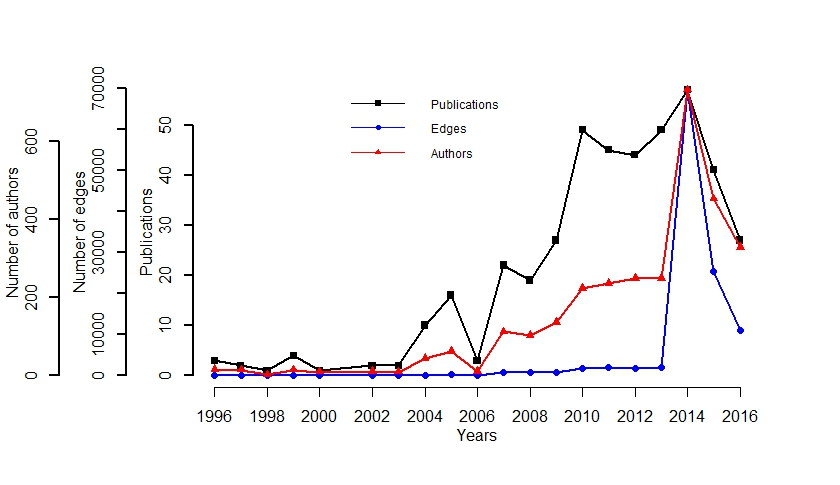
\includegraphics[scale=0.65]{Chapters/malaria/pubDist}
\caption{Evolution of the published Malaria related documents, authors and collaborations from January 1996 to December 2016}
\label{fig: malaria_pubDist}
\end{figure}

\section{Descriptive Data Analysis}
\label{sec:malaria_descstat}
The degrees of the multigraph network range between 1 and 1338 with an average degree distribution of 106.46. We noted in addition, a substantial number of vertices with low degrees (Fig. \ref{malaria_fig1}). There was also a non-trivial number of vertices with higher order of degree magnitudes. A log scale distribution of the degrees demonstrate that the vertex degrees tend to follow a heavy-tail distribution.\\
After we convert the multigraph network in a weighted graph, it results in a simple graph of 1792 vertices and 95,787 weighted edges. Mean Closeness centrality ranges between $3.118\times 10^{-7}$ and $5.152\times 10^{-6}$ with a median of $5.112\times 10^{-6}$. This measure  suggests a highly right-skewed distribution. Betweenness measures range between 0 and 245600 with a median of 1985. A network visualization with the vertices' size proportional to betweenness centrality measures clearly reveals the presence of broker authors (Table \ref{table: malaria_list}). The median eigenvectors measure is 0.005, its  mean is estimated at 0.09. Eigenvectors measures reveal the presence of multiple cluttered authors suggesting the presence of closed collaboration groups. Table \ref{table: malaria_list} presents a list of the 10 authors with the highest Eigenvectors values.

\begin{figure}[!ht]
\centering
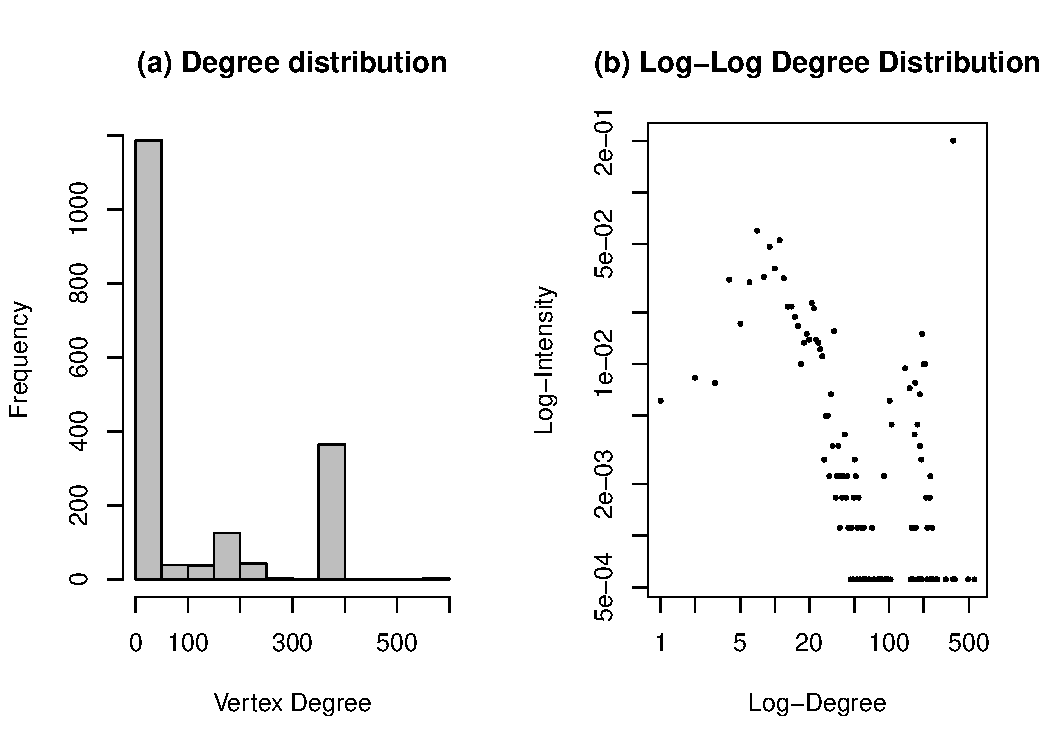
\includegraphics[scale=0.75]{Chapters/malaria/degreeDistribution}
\caption{Degree distribution of the Malaria co-authorship network}
\label{malaria_fig1}
\end{figure}

The computation of edge betweenness identifies co-authorship collaborations that are important for the flow of information. In Table \ref{table: malaria_list}, We present the top 10 most important collaborations for the flow of information in the Malaria co-authorship network in Benin.

%\pagebreak
\begin{table}[!ht]
\caption{List of the most important authors and collaborations in the Malaria co-authorship network}
\label{table: malaria_list}
\centering \scriptsize
\begin{tabular}{l}
  \toprule
\textbf{Top 10 Brokers}\\
%\hline
\hspace{20pt}MASSOUGBODJI ACHILLE\\
\hspace{20pt}HAY SIMON I\\
\hspace{20pt}KAREMA CORINE\\
\hspace{20pt}SANNI AMBALIOU\\
\hspace{20pt}KENGNE ANDRE PASCAL\\
\hspace{20pt}AKOGBETO MARTIN\\
\hspace{20pt}NDAM NICAISE TUIKUE\\
\hspace{20pt}MALIK ELFATIH M\\
\hspace{20pt}DABIRE K ROCH\\
\hspace{20pt}DELORON PHILIPPE\\
\hline
\textbf{Top 10 most connected authors (Top 10 network hubs)}\\
\hspace{20pt}MASSOUGBODJI ACHILLE\\
\hspace{20pt}KAREMA CORINE\\
\hspace{20pt}GONZALEZ RAQUEL\\
\hspace{20pt}MENENDEZ CLARA\\
\hspace{20pt}DALESSANDRO UMBERTO\\
\hspace{20pt}OGUTU BERNHARDS R\\
\hspace{20pt}FAUCHER JEANFRANCOIS\\
\hspace{20pt}BASSAT QUIQUE\\
\hspace{20pt}MARTENSSON ANDREAS\\
\hspace{20pt}HAY SIMON I\\
\hline
\textbf{Top 10 most important edges for information flow}\\
\hspace{20pt}DABIRE K ROCH -- KENGNE ANDRE PASCAL\\
\hspace{20pt}BALDET THIERRY -- KENGNE ANDRE PASCAL\\
\hspace{20pt}AKOGBETO MARTIN -- MALIK ELFATIH M\\
\hspace{20pt}AVLESSI FELICIEN -- MOUDACHIROU MANSOUROU\\
\hspace{20pt}AKOGBETO MARTIN -- AVLESSI FELICIEN\\
\hspace{20pt}MASSOUGBODJI ACHILLE -- RAHIMY MOHAMED CHERIF\\
\hspace{20pt}DIABATE ABDOULAYE -- KENGNE ANDRE PASCAL\\
\hspace{20pt}GARCIA ANDRE -- SANNI AMBALIOU\\
\hspace{20pt}KAREMA CORINE -- MALIK ELFATIH M\\      
\hspace{20pt}HAY SIMON I -- MALIK ELFATIH M\\
\hline
\textbf{Weak articulation points}\\
\hspace{20pt}NOEL VALERIE\\
\hspace{20pt}DJOGBENOU LUC\\
\hspace{20pt}ZOHOUN I\\
\hspace{20pt}SANNI AMBALIOU\\
\hspace{20pt}EDORH ALEODJRODO PATRICK\\
\hspace{20pt}ALLABI AUREL\\
\hspace{20pt}HOUNKONNOU MAHOUTON NORBERT\\
\hspace{20pt}FAYOMI BENJAMIN\\
\hspace{20pt}KINDEGAZARD DOROTHEE A\\
\hspace{20pt}DJOUAKA ROUSSEAU\\
\hspace{20pt}RAHIMY MOHAMED CHERIF\\
\hspace{20pt}BALDET THIERRY\\
\hspace{20pt}DOSSOUGBETE L\\
\hspace{20pt}GARCIA ANDRE\\
\hspace{20pt}MASSOUGBODJI ACHILLE\\
\hspace{20pt}AKOGBETO MARTIN\\
\bottomrule
\end{tabular}
\end{table}

\subsection{Network Cohesion}
A total of 365 maximal cliques are identified in the network among which 9 cliques of size 2, 14 cliques of size 3, 155 cliques of size 8, and 142 cliques of size 7. Larger maximal cliques sizes range from 102 authors to 365 authors and are all found once across the network. \\The malaria co-authorship network has a density of 0.0596 and a transitivity of 0.965 indicating that 96.5\% of the connected triples in the network are close to form triangles. The transitivity metrics is a measure of the global clustering of the network.\\The network is not connected and a census of all the connected components within the network reveals the existence of a giant component that dominates all the other connected components. This giant component includes 94\% (1686 vertices) of all the vertices in the network with none of the other components alone carrying less than 1\% of the vertices in the network (Fig. \ref{malaria_fig5}).  \\The assessment of information flow in the network via cut vertices reveal the existence of 16 authors as the most vulnerable vertices in the network. Table \ref{table: malaria_list} lists the authors that constitute the weak articulation points in the malaria co-authorship network. Cut vertices are crucial to the sustainability of networks \cite{kolaczyk_statistical_2014}.\\
The agglomerative hierarchical clustering method identifies 23 research communities (or clusters) in the network. Sizes of the clusters range between 2 and 570 with large research communities containing between 202 and 569 authors. Medium size research communities contain between 10 and 62 authors. Only 7 out of the 23 research communities identified are part of the giant component. Figure \ref{malaria_fig5} displays the giant component of the network with each different colors representing each of the 7 research communities.

\begin{figure}[!ht]
\centering
\hspace*{-1cm}
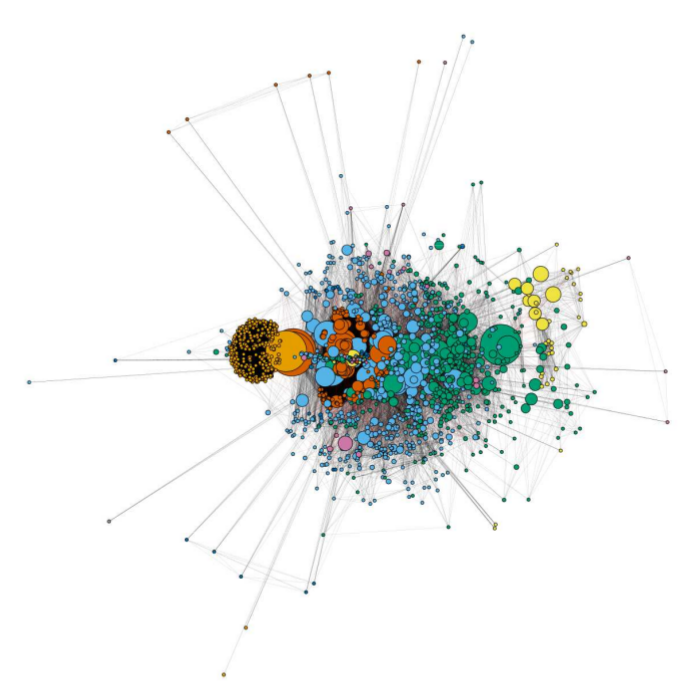
\includegraphics[scale=0.5]{Chapters/malaria/mnet}
\caption{Malaria co-authorship network -- Main component. \\Authors (vertices) of the same color belong to the same research community or cluster}
\label{malaria_fig5}
\end{figure}
\pagebreak
\section{Modeling}
\subsection{Mathematical Modeling}
The hierarchical clustering method of community detection algorithm has identified 23 different clusters/communities in the co-authorship network out of which 7 form a giant component. One of the question of interest in this section is whether the number of communities detected is expected or not. The results of 1,000 Monte Carlo based simulations to test the significance of this observed characteristic are presented on figures \ref{malaria_fig3} and \ref{malaria_fig4}. Figure \ref{malaria_fig3} clearly demonstrates that the number of communities detected is unusual from the perspective of both Classical random graphs and generalized random graphs (p-value < 0.0001). From the Classical random graph model, the expected number of communities is 3.934 (95\%CI: 3.90 -- 3.97). Similarly, the expected number of communities from the generalized random graph model is 7.501 (95\%CI: 7.39 -- 7.61).

\begin{figure}[!ht]
\centering
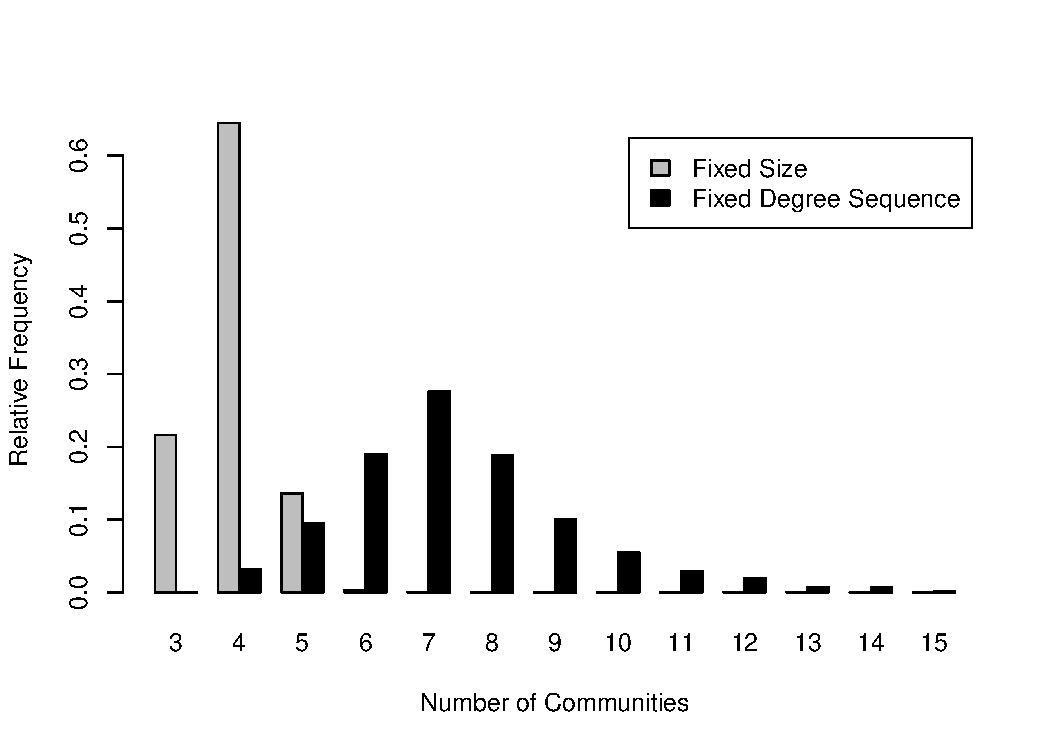
\includegraphics[scale=0.75]{Chapters/malaria/randomComm}
\caption{Monte-Carlo simulations: Number of detected communities by the random graph models}
\label{malaria_fig3}
\end{figure}

Figure \ref{malaria_fig4} displays the number of detected research communities using the Barab\'asi-Albert's preferential attachment and the Watts-Strogatz models. Supprisingly enough, the observed number of communities is also extreme per both models (p-value < 0.0001). The expected number from the Watts-Strogatz model simulations is 3.056 (95\%CI: 3.04 -- 3.07) and 45.569 (95\%CI: 45.42 -- 45.72) from the Barab\'asi-Albert model simulations.

\begin{figure}[!ht]
\centering
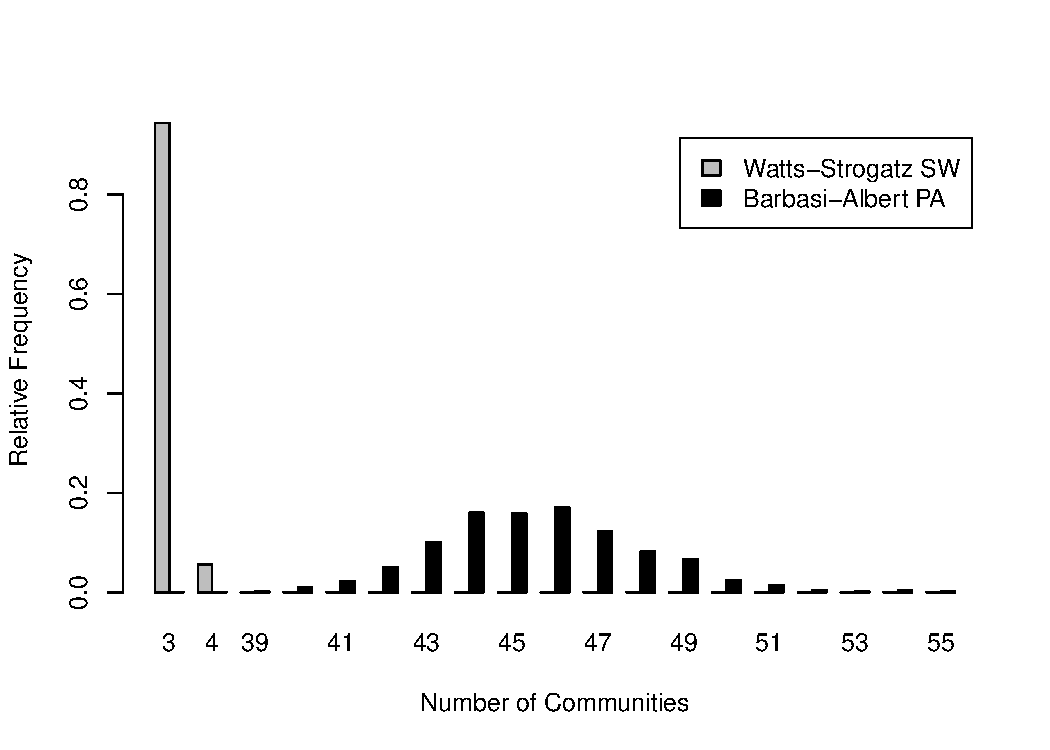
\includegraphics[scale=0.75]{Chapters/malaria/mechanisticComm}
\caption{Monte-Carlo simulations: Number of detected communities by the Watts-Strogatz and the Barab\'asi-Albert models}
\label{malaria_fig4}
\end{figure}

We also compared the clustering coefficient and the average shortest-path length. The observed clustering coefficient is 0.9645. Surprisingly, there is substantially more clustering in our malaria co-authorship network than expected from all 4 mathematical models (p-value < 0.0001). The expected clustering coefficient is 0.0596 (95\%CI: 0.05963068 -- 0.05964648) and 0.4334 (95\%CI: 0.4333912 -- 0.4334522) respectively for the classic random graph and the generalized random graph models.\\
Similarly, The Watts-Strogatz Small World model expected clustering is 0.7464 (95\%CI: 0.7464326 -- 0.7464356).\\
We observed an average shortest-path length of 2.99 in the malaria co-authorship network. This observed shortest-path length is significantly larger than what is expected from the random graph models (p-value < 0.0001) and significantly lower than what is expected from Watts-Strogatz small world model and the Barab\'asi-Albert preferential attachment model (p-value < 0.0001).\\The average shortest-path length is 1.94 (95\%CI: 1.941955 -- 1.941960) and 2.26 (95\%CI: 2.259468 2.259586) respectively for the classic random graph and the generalized random graph models.\\For the Watts-Strogatz small world and the Barab\'asi-Albert models, the average shortest-path length is respectively 3.83 (95\%CI: 3.81 -- 3.86) and 9.17 (95\%CI: 9.14 -- 9.21).\\~\\
All simulations were also performed on the giant component of the network and led to similar outcomes.%\\

\subsection{Statistical Modeling}
\subsubsection{Stochastic Block Model}
\label{sec:malaria_results_sbm}
The ICL plot on figure \ref{fig:malaria_sbmgof} shows that the malaria co-authorship network has been fit with 39 classes by the SBM with a degree of latitude of 30 to 39 classes being reasonable. The degree distribution of the fitted SBM (blue curve) provides a decent description of the observed distribution (yellow histogram). In the inter/intra class probabilities network, the vertices correspond to the 39 classes detected by the SBM. The vertex sizes are proportional to the number of authors assigned to each class. Each vertex is further broken down in a pie chart with each portion reflecting the relative proportion of the types of collaboration. Yellow represents the proportion of authors of international affiliations, orange represents regional authors who are affiliated with African institutions other than Beninese institutions, and green for authors affiliated to Beninese research institutions. In general, we observe a dominance of international and regional researchers over national researchers across all detected clusters.

\begin{figure}[!ht]
\centering
%\definecolor{shadecolor}{rgb}{0.969, 0.969, 0.969}\color{fgcolor}
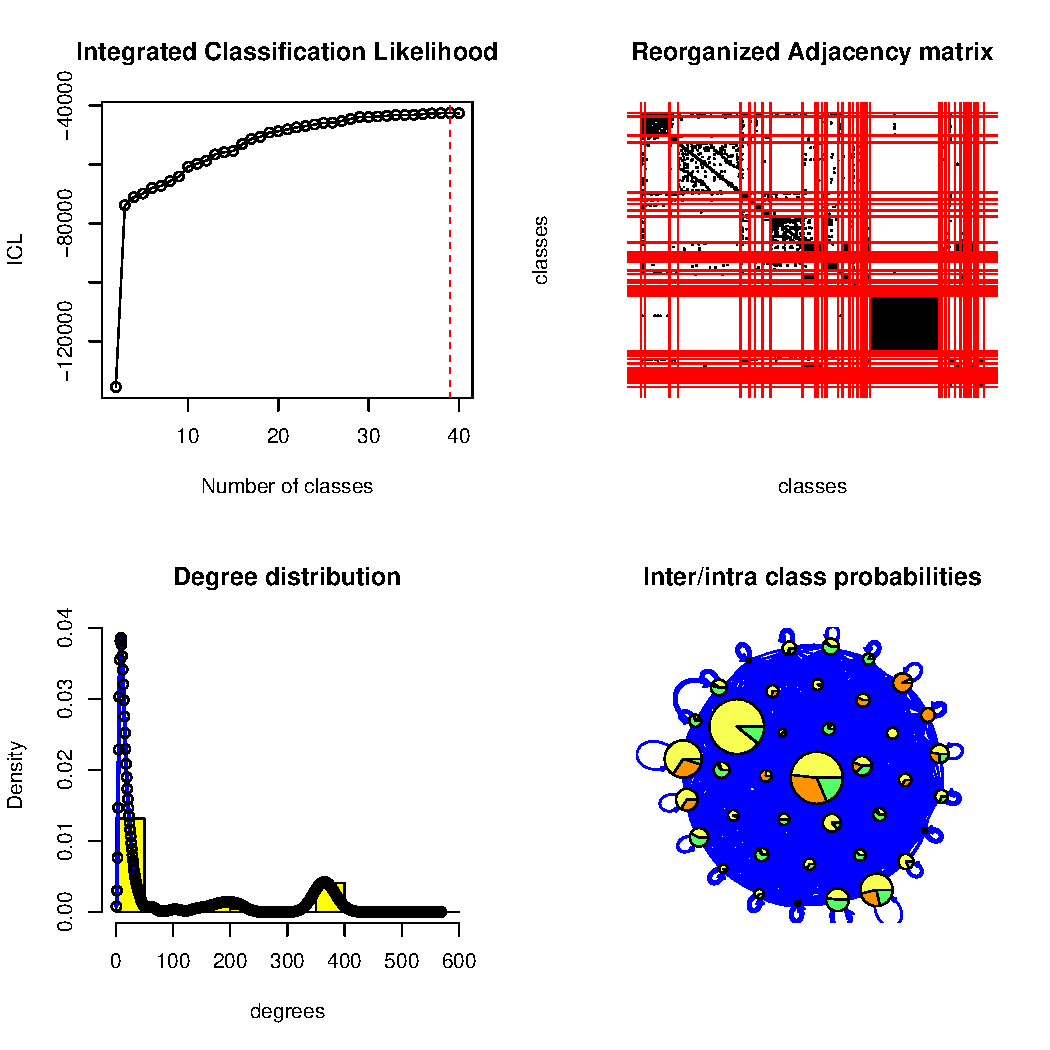
\includegraphics[scale=0.75]{Chapters/malaria/statMod/unnamed-chunk-1-1}
\caption{Summary of the goodness-of-fit of the SBM analysis on the Malaria co-authorship network.
%The SBM model was fit with 39 classes with a latitude of between 30 and 39 classes being reasonable.
}
\label{fig:malaria_sbmgof}
\end{figure}

A close look at the reorganized adjacency matrix, reveals the presence of 4 larger classes (classes number 2, 4, 10 and 27) and 35 other classes of smaller sizes. One of the larger class (class 27) displays a tendency of its members to only establish collaboration ties between themselves. This class seems to have the characteristics of a clique. Examination of the distribution of each class by their type of collaboration (Figure \ref{fig:malaria_dist}) indicates that this class of authors (class 27) is primarily made of international contributors to the malaria research effort in Benin. Although members of this class seem to have rare collaboration ties with members of other classes, we also notice the presence of very few broker authors as national liaisons between this class 27 and another larger class (class 2). Though, it also appears in the other three larger classes that the authors tend to primarily collaborate within their respective classes, they also tend to collaborate with authors of other classes.

\begin{figure}[!ht]
\centering
%\definecolor{shadecolor}{rgb}{0.969, 0.969, 0.969}\color{fgcolor}
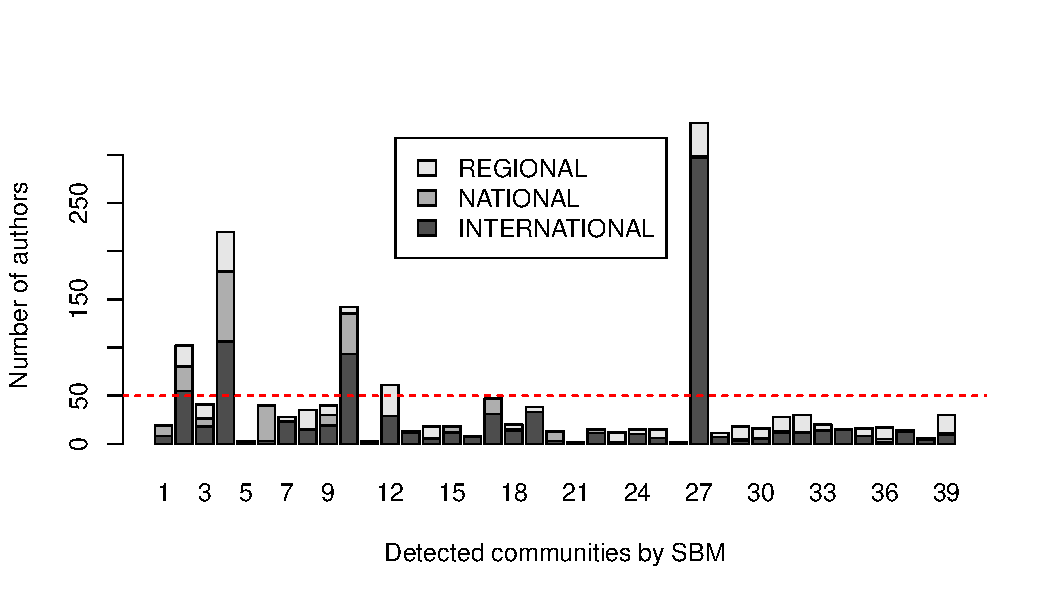
\includegraphics[scale=0.75]{Chapters/malaria/statMod/unnamed-chunk-2-1}
\caption{Distribution of national, international and regional authors by communities detected by the SBM in the Malaria network.}
\label{fig:malaria_dist}
\end{figure}

Figure \ref{fig:malaria_dist} also shows that the co-authorship malaria network in Benin is dominated by international researchers with national contributors unevenly distributed across the detected research communities. In order to better explain the inter/intra class interactions, we highlight in figure \ref{fig:malaria_sbmgof2}, the main classes driving the structure of the network. We present the results from the SBM on the classes with 50 authors or more. This reorganization clearly confirmed the presence of a clique of mainly international contributors who tend to collaborate rarily outside their class. The larger size here (Figure \ref{fig:malaria_sbmgof2}) is very diversed and contains all regional contributors to the malaria research effort. The presence of 3 smaller cliques which collaborate intensively between themselves is worth noting as well (See inter/intra class probabilities network on figure \ref{fig:malaria_sbmgof2}).

\begin{figure}[!ht]
%\definecolor{shadecolor}{rgb}{0.969, 0.969, 0.969}\color{fgcolor}
\centering
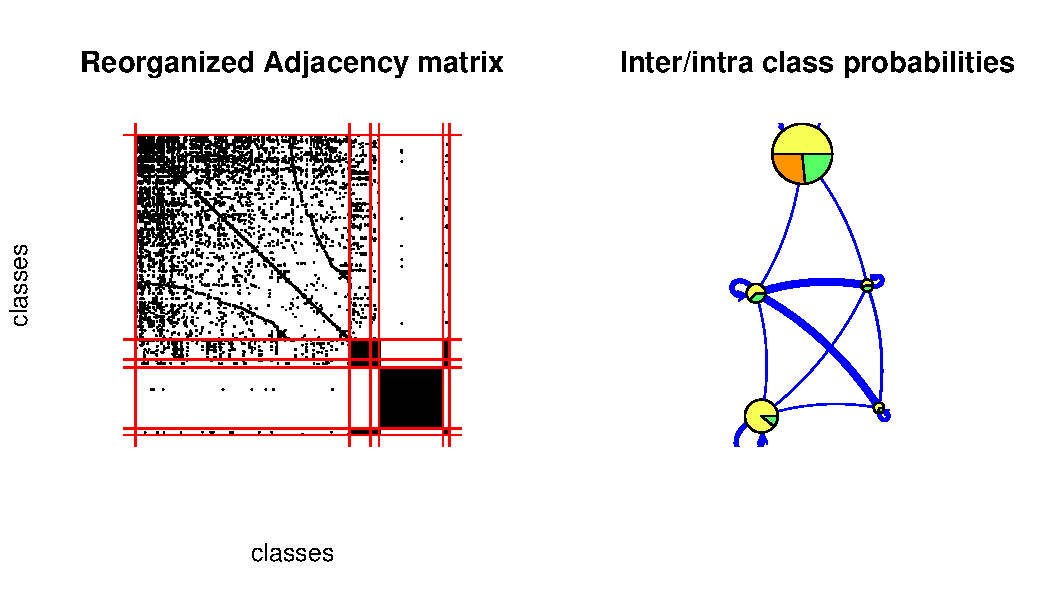
\includegraphics[scale=0.75]{Chapters/malaria/statMod/unnamed-chunk-3-1}
\caption{Summary of the goodness-of-fit of the SBM analysis highlighting interactions between the top 5 larger classes of the Malaria co-authorship network.}
\label{fig:malaria_sbmgof2}
\end{figure}
%
%\subsubsection{Dynamic Stochastic Block Model}
%%\label{sec:results_dynsbm}
%Figure \ref{fig:malaria_ICL} represents variation in ICL and log-likelihood by the number of detected research groups or communities by the dynSBM. The optimal number of groups determined by the ICL criterion is 14. However, the "elbow" heuristic suggests 5 detected groups. We therefore, ended up choosing the final dynSBM with 5 detected groups.
%
%\begin{figure}[!ht]
%%\definecolor{shadecolor}{rgb}{0.969, 0.969, 0.969}\color{fgcolor}
%\hspace{-1cm}
%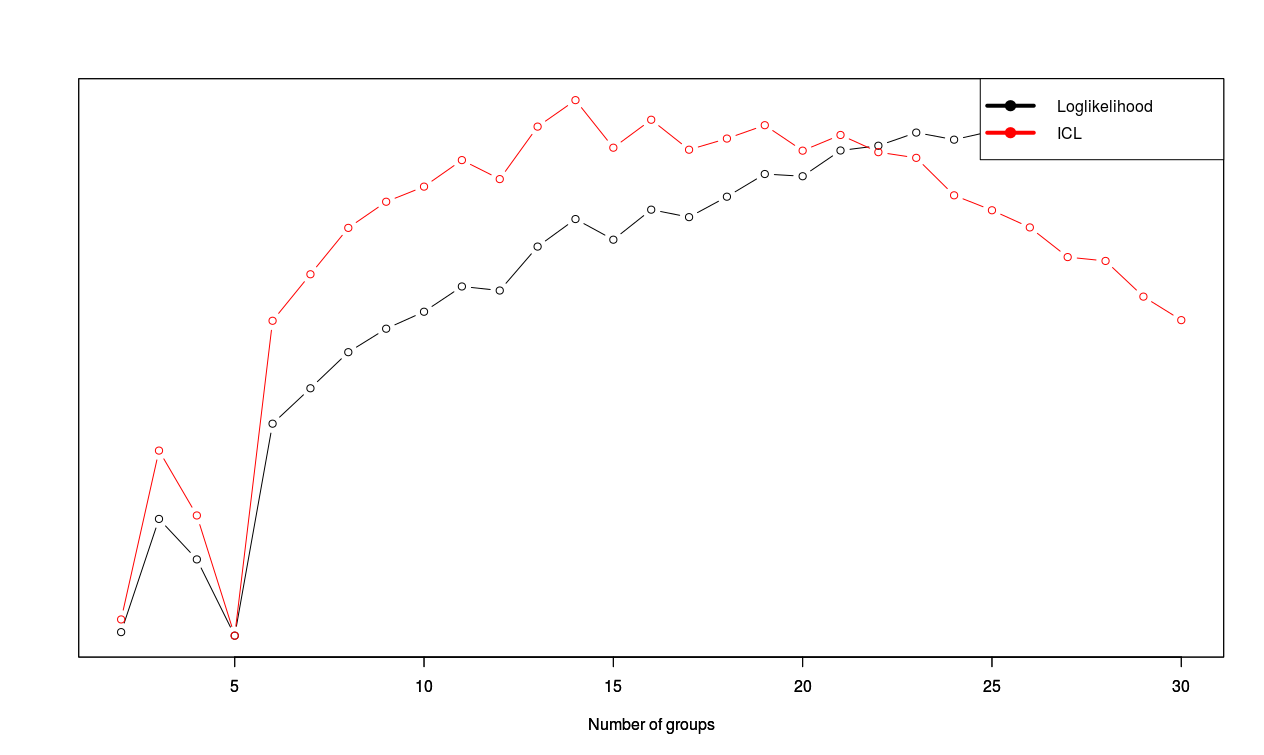
\includegraphics[scale=0.5]{Chapters/malaria/statMod/ICL_plot1}
%\caption{ICL and log-likelihood by number of detected research groups/communities.}
%\label{fig:malaria_ICL}
%\end{figure}
%
%Figure \ref{fig:malaria_connectivity} displays the structure of the dynamic network through the symmetric inter/intra group interaction properties. Interactions present in the figure are between nodes in any of the 5 detected groups to the others via a global $Q \times Q$ matrix. Each cell contains $T=7$ time points on the x-axis corresponding to the different time steps described in section \ref{sec:malaria_data}. As our network only contains binary edges, only interaction present is represented by the blue area. The $Q \times Q$ matrix shows directed interaction from group $q$ (rows) to group $l$ (columns). It is clear that intra-group interactions are more frequent across the study period, particularly in group 1, 3 and 5. For groups 1 and 5, this pattern appears stable in time while for group 3, it seems to have declined in the year 2014 followed by an upward trend in 015 and 2016. About inter-group collaboration ties establishment, the most striking pattern concerns authors in group 1 who tend to collaborate with authors in group 3. While this pattern seems unstable across the time steps, we note however an upward trend starting in 2014. Another important observation made here is the low inter-group interaction in group 2. Inter-group interaction in group 4 appears very unstable with some peaks in in 2007--2009 and in 2015.
%%We assess whether all authors have the same propensity to establish collaboration ties from one group to another one. Our observations suggest that globally, the average probability of between group collaboration ties establishment is estimated at 20\% across the 20 years of longitudinal network data.
%
%\begin{figure}[!ht]
%%\definecolor{shadecolor}{rgb}{0.969, 0.969, 0.969}\color{fgcolor}
%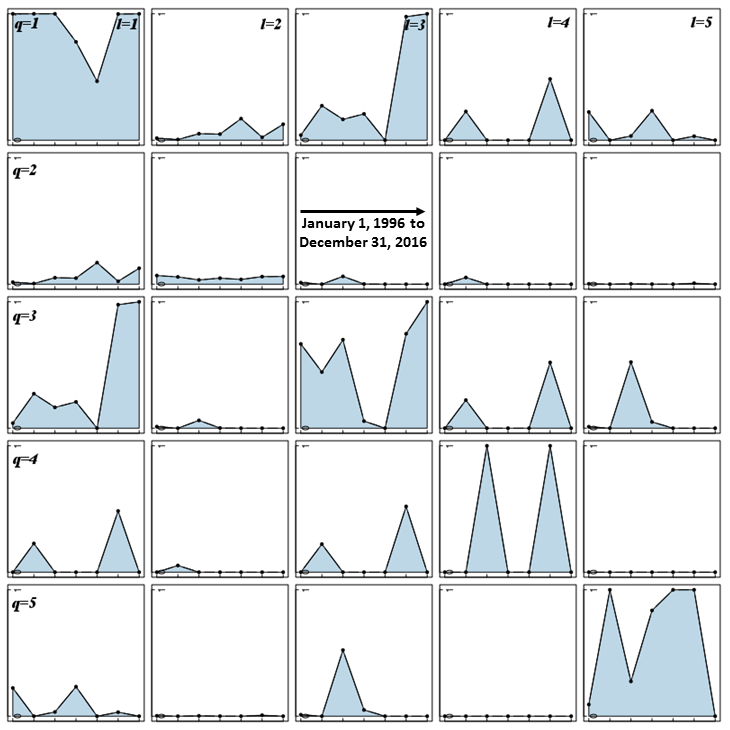
\includegraphics[scale=0.75]{Chapters/malaria/statMod/cPlot_q5}
%\caption{Interaction properties between research groups/communities in the Malaria co-authorship network.}
%\label{fig:malaria_connectivity}
%\end{figure}
\pagebreak
\subsubsection{Exponential Random Graph Model}
\label{sec:malaria_results_ergm}
Table \ref{tab:malaria_ergm} summarizes the results of the different models we fit to the observed network. Model 1 is analogous to the null model in a typical General Linear Model (GLM). The probability of any two authors establishing a collaboration tie is therefore expressed as the inverse logit of the edge coefficient. The inverse logit of a coefficient $x$ is defined as $logit^{-1}(x)=1/(1+exp(-x))$. The conditional log-odds for a collaboration between authors in the network is $-2.76$. The associated probability of any two authors establishing a collaboration tie is therefore $5.96\%$. To put this in perspective, this probabibility is the same as the density of the malaria co-authorship network. Since, our network is characterized by a high transitivity, we modeled the triangle ERGM term along with the edge term in model 2. We see some improvements in the model performance with a significantly positive but small triangle effect on the collaboration tie formation (Coefficient $= 0.08$, $p<0.001$). \\
In model 3, we describe the co-authorship network as a function of the number of collaborations, the number of publications, and the number of citations of authors inside the network. We also include confounding homophily term on cluster assignment from the SBM and on the collaboration type. Compared to models 1 and 2, model 3 has tremendously improved (See AIC and BIC in table \ref{tab:malaria_ergm}). The edge effect has decreased (Coefficient $=-7.98$, $p<0.001$) with the associated conditional probability (given all other terms in the model) equal to $0.03\%$. We observed a small, though positively significant effect of the number of collaborators and the number of publications on the odds of collaboration tie formation between any two authors. One unit increase in the number of collaborators increases the odds of collaboration tie by $2\%$ while one unit increase in the number of publications increases the odds of establishing a collaboration tie by $12.75\%$. On the other hand, model 3 has found a very small but significant negative effect of the number of times an author was cited on the odds of collaboration tie formation. One unit increase in the number of citation of a given author was associated with 1\% decrease in the odds of collaboration between two authors conditional on all the other terms in the model. \\
It clearly appears that the process underlying the malaria co-authorship network is driven by homophily on cluster assignment or membership to a specific research community and the type of collaboration. The conditional probability of two authors collaborating adjusted by the homophily on their membership to a research community is estimated at $8.32\%$ compared to the baseline probability of $0.03\%$ given all other terms in model 3. Adjusted by the collaboration type, the same probability is estimated at $0.05\%$ conditional on all other terms in the model. The overall conditional probability adjusting for all terms in model 3 is estimated at $14.06\%$ which is a lot greater than the $5.95\%$ estimated from model 1.\\
In model 4, we introduced  factor attributes on the collaboration type in order to investigate the likelihood of researchers affiliated to Beninese institutions to establish international and regional or African collaboration ties. While model 4 slightly improved upon model 3, it displays minor changes in the coefficient of the terms it has in common with model 3. Overall, compared to researchers with international research affiliations, researchers affiliated to Beninese research institutions have $37.7\%$ average decrease in the odds of establishing collaboration ties. On the other hand, researchers affiliated to other African research institutions have $78.6\%$ increase in the odds of establishing a collaboration tie than researchers affiliated to international research institutions. In other words, in model 4, the probability for researchers affiliated to international institutions to establish a collaboration tie is estimated at $14.19\%$, that of researchers affiliated to Beninese institutions is $10.72\%$, and that of researchers affiliated to African institutions other than Beninese institutions is $22.79\%$. \\
None of the structural models containing high order ERGM terms, nor the models containing the dyadic attribute terms converged after the maximum of 1,000 iterations making estimates from these models unreliable. This observation justifies the reason why we do not present the results from these models in table \ref{tab:malaria_ergm}. The unability of model containing structural terms to converge also makes it impossible for us to assess model degeneracy as recommended by Handcock et al. \cite{handcock_assessing_2003}.

\begin{table}[!h]
\caption{ERGM of the co-authorship Malaria network.} \scriptsize
\label{tab:malaria_ergm}
\hspace*{-1.5cm}
      \begin{tabular}{@{}lcclclclcl@{}}
        \toprule
           &  & Model 1 &  & Model 2  &  & Model 3&  & Model 4\\ \cmidrule{3-3} \cmidrule{5-5} \cmidrule{7-7} \cmidrule{9-9}
           &  & Estimate ($SE$) &  & Estimate ($SE$)  &  & Estimate ($SE$) &  & Estimate ($SE$)\\ \midrule
        Network structural predictor &  &   &  &  &  & &  & \\
        \hspace{10pt}Intercept(edge) &  & $-2.76\hspace{2pt}(0.00)^{***}$  &  & $-5.00\hspace{2pt}(0.01)^{***}$   &  & $-7.98\hspace{2pt}(0.02)^{***}$ &  & $-8.22\hspace{2pt}(0.02)^{***}$\\
        \hspace{10pt}Triangle &  & --   &  & $\hspace{6pt}0.08\hspace{2pt}(0.00)^{***}$   &  & --  &  & --\\ \\
        %\hspace{10pt}Degree &  & --   &  & --     &  & --  &  & --\\ \\
        Number of collaborations &  & --   &  & --  &  & $\hspace{6pt}0.02\hspace{2pt}(0.00)^{***}$  &  & $\hspace{6pt}0.01\hspace{2pt}(0.00)^{***}$\\% \\
        Number of publications &  & --   &  & --  &  & $\hspace{6pt}0.12\hspace{2pt}(0.00)^{***}$  &  & $\hspace{6pt}0.13\hspace{2pt}(0.00)^{***}$\\% \\
        Number of times cited &  & --   &  & --   &  & $-0.01\hspace{2pt}(0.00)^{***}$  &  & $-0.01\hspace{2pt}(0.00)^{***}$\\% \\
        Homophily on cluster assignment &  & --   &  & --    &  & $\hspace{6pt}5.58\hspace{2pt}(0.02)^{***}$  &  & $\hspace{6pt}5.68\hspace{2pt}(0.02)^{***}$\\% \\
        Homophily on collaboration type &  & --   &  & --    &  & $\hspace{6pt}0.46\hspace{2pt}(0.01)^{***}$  &  & $\hspace{6pt}0.61\hspace{2pt}(0.00)^{***}$\\ \\
        Factor attribute effect (collaboration type) &  &    &  &  &   &  &  & \\
        \hspace{10pt}International &  & --   &  & --   &  & --  &  & $REF$\\
        \hspace{10pt}National &  & --   &  & --   &  & --  &  & $-0.32\hspace{2pt}(0.02)^{***}$\\
        \hspace{10pt}Regional &  & --   &  & --   &  & --   &  & $\hspace{6pt}0.58\hspace{2pt}(0.01)^{***}$\\ \\ \midrule
        Number of iterations  &   & $6$   &  & $18$ &  & $8$  &  & $9$\\
        Akaike's Information Criterion (AIC)  &   & $725268$   &  & $660444$ &  & $220964$  &  & $217026$\\
        Bayesian Information Criterion (BIC)  &   & $725280$   &  & $660469$ &  & $221038$  &  & $217125$\\
        Model Log Likelihood  &   & $-362633$ ($df=1$)   &  & $-330220$ ($df=2$) &  & $-110475.9$ ($df=6$)  &  & $-108505.2$ ($df=8$)\\
        \bottomrule
      \end{tabular}
      \hspace*{-1cm}
      \raggedright \scriptsize
      $REF=$ reference, $SE=$ Standard Error, $df=$ degree of freedom\\
      ${ }^{***} p < .001$\\
      ${ }^{\hspace{3pt}**} p < .01$\\
      ${ }^{\hspace{5pt}*} p < .05$
\end{table}

Figure \ref{fig:malaria_ergm-gof} presents the goodness-of fit of model 4. The observed properties are depicted by the black lines. Gray lines with circles represent the 95\% confidence intervals for the simulated network properties. Goodness-of-fit is asserted when the black lines lie in-between the confidence intervals lines. The wide range of degree distribution of our co-authorship network makes it difficult to assess model fit in terms of degree distribution. But it is clear that in general, model 4 fits poorly to the observed network despite the highly significant estimates obtained. We therefore have strong evidence confirming that there is likely something other than the terms included in this model that are driving the structure of the network, possibly additional attributes our study did not control for. The following section attempts to address this shortcoming.

\begin{figure}[!h]
\centering
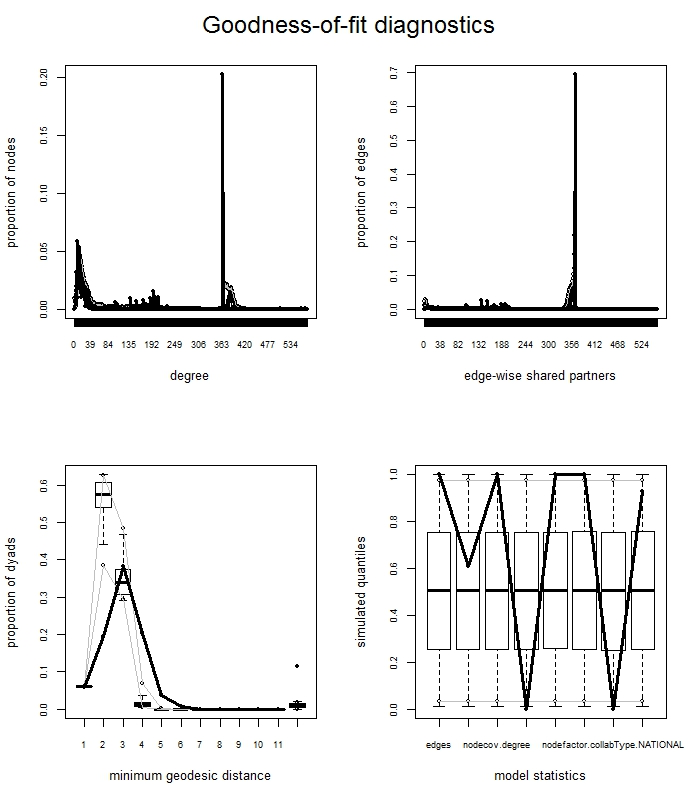
\includegraphics[scale=0.65]{Chapters/malaria/statMod/ergm_gof}
\caption{ERGM goodness-of-fit of final model 4 assessment.\\
%The observed properties are depicted by the black lines. Gray lines with circles represent the 95\% confidence intervals for the simulated network properties. Goodness-of-fit is asserted when the black lines lie in-between the confidence intervals lines.
}
\label{fig:malaria_ergm-gof}
\end{figure}

\pagebreak
\subsubsection{Temporal Exponential Random Graph Model}
\label{sec:malaria_results_tergm}
The observed cumulative network was subset in seven snapshots representing respectively the following time spans: 1996 -- 2006, 2007 -- 2009, 2010 -- 2011, 2012 -- 2013, 2014, 2015 and 2016. %\\
Figure \ref{fig:malaria_dynNetwork} displays the topological structure of the snapshots of the different time steps.

\begin{figure}[!ht]
\hspace{-1.25cm}
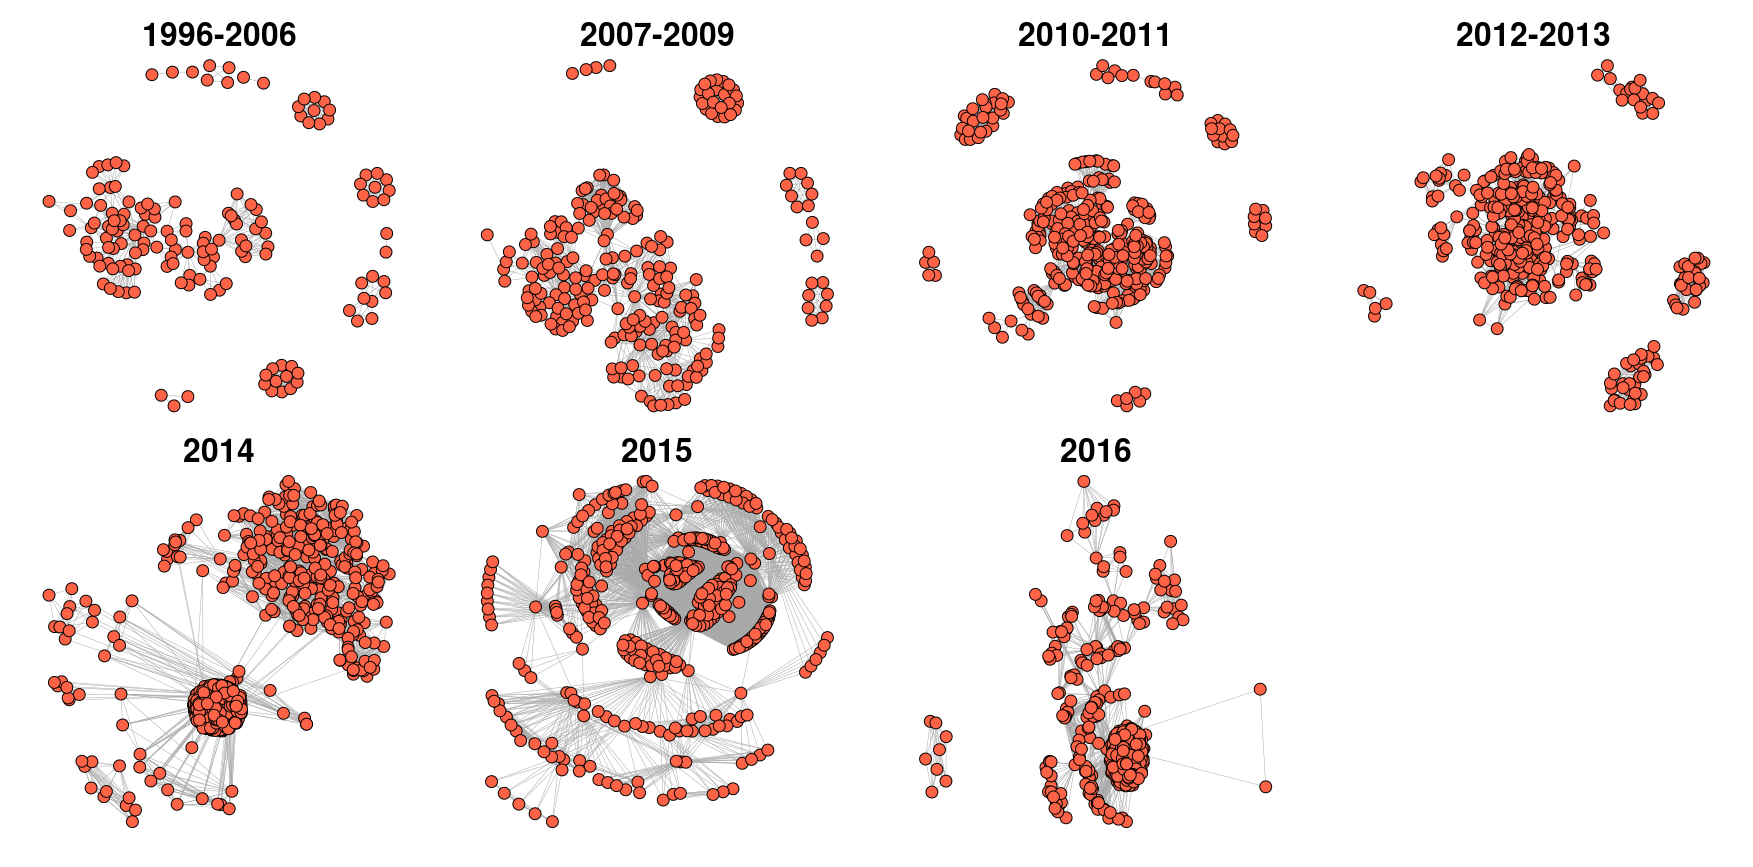
\includegraphics[scale=0.4]{Chapters/malaria/statMod/dynMNet2}
\caption{Topological structure of the different snapshots of the malaria co-authorship network.}
\label{fig:malaria_dynNetwork}
\end{figure}

Table \ref{tab:malaria_tergm} summarizes the results of the different temporal models we fit to the observed network. Models 1, 2, and 3 are equivalent to a pooled ERGM across the 7 different time points (Fig. \ref{fig:malaria_dynNetwork}). The null model of the TERGM (model 1) suggests that the baseline log-odds for collaboration tie formation between authors in the network is $-4.66$. This coefficient is equivalent to a baseline probability of $0.9\%$ for any two authors in the network to establish a stable collaboration tie. This probability is significantly lower than the 5.96\% baseline probability of collaboration tie establishment reported by the ERGM (section \ref{sec:malaria_results_ergm}). \\
Model 2 of the TERGM describes the co-authorship network as a function of the number of collaborations, the number of publications, and the number of citations of authors inside the network. It is also adjusted by homophily on cluster assignment from the SBM and on the collaboration type. Compared to model 1, model 2 has slightly improved (See AIC and BIC in table \ref{tab:malaria_tergm}). The edge effect has decreased (Coefficient $=-10.14$, $p<0.001$) with the associated conditional probability (given all other terms in the model) equal to $0.004\%$. We observed a relatively high positively significant effect of the homophily on cluster assignment on the odds of collaboration tie formation between any two authors. Adjusting for the other variables in model 2, authors of the same research groups/communities are $4.96$ times as likely to collaborate than authors that belong to different research groups. The effect of the other attributes in model 2 are minor. When we adjust for attribute effect on the collaboration type, we obtained model 3 which is slightly better than model 2. Relatively to model 2, the edge effect decreases more followed by an even stronger effect of the homophily on cluster assignment of the authors in the network (Coefficient $=5.06$, $p<0.001$). \\
After introducing temporal dependencies terms, we obtained model 4 which tremendously improved compared to models 1, 2 and 3. Model 4 confirms the observation made in section \ref{sec:malaria_results_ergm} that the process underlying the malaria co-authorship network is driven by homophily on cluster assignment or membership to a specific research community and the type of collaboration. It further confirms that the linear trend suspected observed in figure \ref{fig: malaria_pubDist} is significantly associated with the odds of collaboration tie formation in the Malaria co-authorship network. Model 4 suggests that the baseline conditional probability of any two authors to collaborate is estimated at 0.02\% given all other terms in the model. The coefficient associated to the dyadic stability term is 1.07 meaning that the odds of existent and non existent collaboration ties at one time point to remain the same at the next time point increased on average by $65.7\%$. In other words, the odds of new collaboration ties and non-ties to occur from one time point to another is $34.3\%$. In addition, the TERGM showed that the probability of sustainable collaboration tie formation among international researchers is $12.13\%$ versus $12.24\%$ for researchers affiliated with national institutions ($p>0.05$). However, this probability significantly increases to $20.26\%$ for researchers affiliated to African research institutions other than those in Benin. These probabilities confirm the results from the ERGM final model with respect to the higher probability of tie formation between researchers affiliated to African institutions other than Beninese institutions. None of the structural temporal models containing high order TERGM terms, nor the models containing the dyadic attribute terms converged after the maximum of 1,000 iterations making estimates from these models untrustful.\\

\begin{table}[!h]
\begin{center}
\caption{Temporal ERGM of Malaria co-authorship network.}
\label{tab:malaria_tergm}
\hspace*{-1cm}
\scriptsize
\begin{tabular}{@{}lcclclclcl@{}}
        \toprule
           &  & Model 1 &  & Model 2  &  & Model 3&  & Model 4\\ \cmidrule{3-3} \cmidrule{5-5} \cmidrule{7-7} \cmidrule{9-9}
           &  & Estimate ($SE$) &  & Estimate ($SE$)  &  & Estimate ($SE$) &  & Estimate ($SE$)\\ 
        \midrule
Network structural predictor & & & & & & & & \\
\hspace{10pt}Intercept(edge)   &  & $-4.66 \; (0.00)^{***}$ &  & $-10.14 \; (0.02)^{***}$ &  & $-10.45 \; (0.02)^{***}$ &  & $-8.65 \; (0.05)^{***}$ \\ \\
Number of collaborations          &  & --  &  & $\hspace{6pt}0.03 \; (0.00)^{***}$  &  & $\hspace{6pt}0.03 \; (0.00)^{***}$  &  & $\hspace{6pt}0.03 \; (0.00)^{***}$  \\
Number of times cited   &  & -- &  & $-0.03 \; (0.00)^{***}$ &  & $-0.02 \; (0.00)^{***}$ &  & $-0.03 \; (0.00)^{***}$ \\
Number of publications  &  & --  &  & $\hspace{6pt}0.45 \; (0.00)^{***}$  &  & $\hspace{6pt}0.46 \; (0.00)^{***}$  &  & $\hspace{6pt}0.45 \; (0.00)^{***}$  \\
Homophily on cluster assignment  &  & --  &  & $\hspace{6pt}4.96 \; (0.02)^{***}$  &  & $\hspace{6pt}5.06 \; (0.02)^{***}$  &  & $\hspace{6pt}4.79 \; (0.02)^{***}$  \\
Homophily on collaboration type   &  & --  &  & $\hspace{6pt}0.44 \; (0.01)^{***}$  &  & $\hspace{6pt}0.56 \; (0.01)^{***}$  &  & $\hspace{6pt}0.54 \; (0.01)^{***}$  \\ \\
Factor attribute effect (collaboration type) & & & & & & & & \\
\hspace{10pt}International & & -- & & -- & & $REF$ & & $REF$ \\
\hspace{10pt}National &  & -- &  & -- &  & $-0.10 \; (0.02)^{***}$        &  & $\hspace{6pt}0.01 \; (0.02)^{~~~~}$        \\
\hspace{10pt}Regional &  & -- &  & --  &  & $\hspace{6pt}0.55 \; (0.01)^{***}$  &  & $\hspace{6pt}0.60 \; (0.01)^{***}$  \\ \\
Temporal dependencies & & & & & & & & \\
\hspace{10pt}Dyadic stability          &  & --  &  & --  &  & --  &  & $\hspace{6pt}1.07 \; (0.01)^{***}$  \\
\hspace{10pt}Linear trends        &  & -- &  & -- &  & -- &  & $-0.18 \; (0.01)^{***}$ \\
%\hspace{10pt}Delayed reciprocity        &  &  -- &  & -- &  & -- &  & NA \\
\midrule
Akaike's Information Criterion (AIC)  &  & $\hspace{6pt}94681198$ &  & $\hspace{6pt}93740511$ &  & $\hspace{6pt}93737596$ &  & $\hspace{6pt}67005816$           \\
Bayesian Information Criterion (BIC)  &  & $\hspace{6pt}94681230$ &  & $\hspace{6pt}93740624$           &  & $\hspace{6pt}93737742$ &  & $\hspace{6pt}67005991$           \\
Model Log Likelihood &  & $-47340597$ &  & $-46870248$ &  & $-46868789$ &  & $-33502897$   \\
\bottomrule
%\multicolumn{5}{l}{\scriptsize{$^{***}p<0.001$, $^{**}p<0.01$, $^*p<0.05$}}
\end{tabular}
      \hspace*{-1cm}
      \raggedright \scriptsize
      $REF=$ reference, $SE=$ Standard Error\\
      ${ }^{***} p < .001$\\
      ${ }^{\hspace{3pt}**} p < .01$\\
      ${ }^{\hspace{5pt}*} p < .05$
\end{center}
\end{table}

Figure \ref{fig:malaria_tergm-gof} presents the goodness-of-fit assessment for the TERGM model 4. We can see that this model containing temporal dependencies fits better to the observed Malaria co-authorship network than the final ERGM model 4. While the first five subfigures compare the distribution of endogenous network statistics between the observed network and the simulated ones, the last subfigure presents the Receiver Operating Characteristics (ROC) and precision-recall (PR) curves. In general, the closer the curve is to the left-hand border and the top border of the ROC space, the more accurate the prediction is. On the other hand, the closer the curve is to the 45-degree diagonal of the ROC space, the less accurate is the prediction. The ROC for model 4 is depicted by the dark red curve compared to the ROC of a random graph depicted by the light red curve. Similarly, the dark blue curve represents the PR of model 4 versus the light blue curve representing the PR of a random graph \cite{leifeld_temporal_2015}. It clearly appears that the final TERGM model 4 outperformed the random null model with an Area Under the Curve (AUC) value estimated at $79.98\%$.

\begin{sidewaysfigure}
%\begin{figure}[!h]
\centering
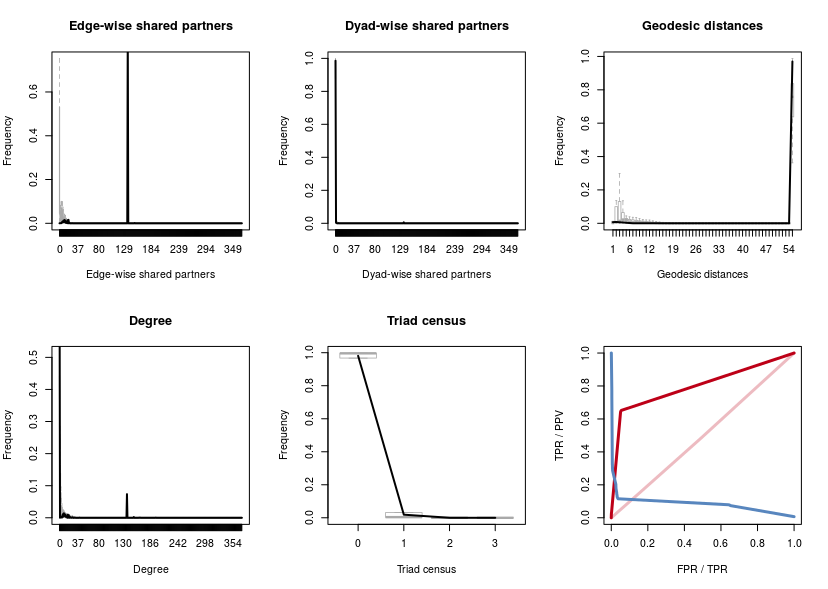
\includegraphics[scale=0.9]{Chapters/malaria/statMod/tergm_gof}
\caption{Goodness-of-fit assessment for the final Malaria TERGM Model 4 with temporal dependencies.}
\label{fig:malaria_tergm-gof}
%\end{figure}
\end{sidewaysfigure}
%~\\
\pagebreak
\subsubsection{Latent Network Model}
\label{malaria_sec:results_lnm}
Figure \ref{fig:malaria_lnm_viz} presents a 3-dimensional visualization of the Malaria co-authorship network, with layouts determined according to the inferred latent eigenvectors from the no pair-specific model (on top), the model containing nodal covariates (middle), and the model containing nodal and dyadic covariates (bottom). Blue vertices represent authors affiliated to Beninese research institutions, Red vertices are authors affiliated to international institutions, Gold vertices represent authors affiliated to African research institutions other than Benin, and White vertices represent authors with no determined affiliations. Node sizes are proportional to the betweenness value of each vertex. Looking at the three visualizations, it clearly appears that the first two visualizations are somewhat similar while the third is different. In fact, in the first two visualizations, the authors are clustered in mainly three clusters. We can see that all the authors affiliated to Beninese research institutions (in blue) are clustered in one cluster while authors with international affiliations (in red) and regional authors (in gold) are distributed across all three main clusters. These observations suggest a significant geography effect on the odds of collaboration tie establishment in the malaria co-authorship network. \\The first two visualizations also highlight key brokers that liaison between clusters. 
%%%Added from suggested corrections
%%From the WOS API, those key brokers also appears to be the authors with the highest citation count. For example, in the first two visualizations on figure \ref{fig:malaria_lnm_viz}, the brokers with affiliations to national institutions are MASSOUGBODJI ACHILLE, AKOGBETO MARTIN, and SANNI AMBALIOU. These authors are also the ones with the highest citation counts. Such an observation is not surprising given their long tenure, their publication records, and known expertise in malariology.
%%%
In the third visualization, on the other hand, there appears to be only one main cluster. This last observation suggests that the nodal covariates and mainly homophily on research community membership and type of affiliation explain much less coarse-scale network compared to dyadic covariates. Indeed, when the dyadic covariates are added to the model, there is less structure left to be captured by the latent variables. These results compensate the lack of-fit of the ERGM model and confirmed our findings in the previous section.

\begin{figure}[!h]
\center
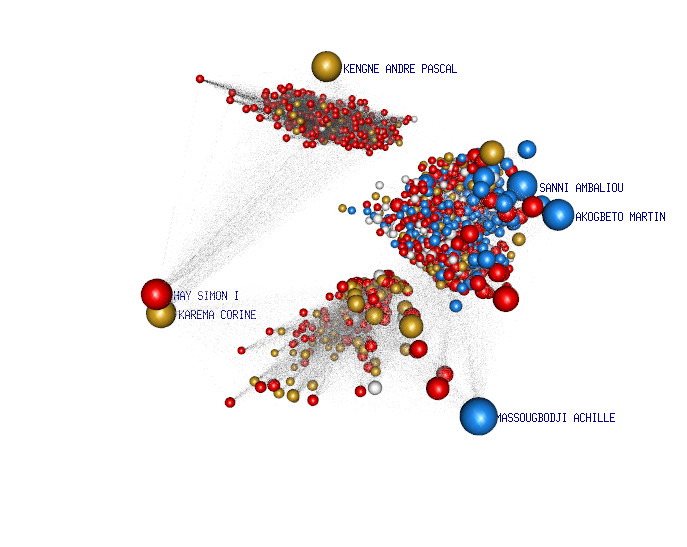
\includegraphics[scale=0.3,trim={5cm 0 0 0}]{Chapters/malaria/statMod/lnm_mod1_null.png}
\vspace{0px}\\
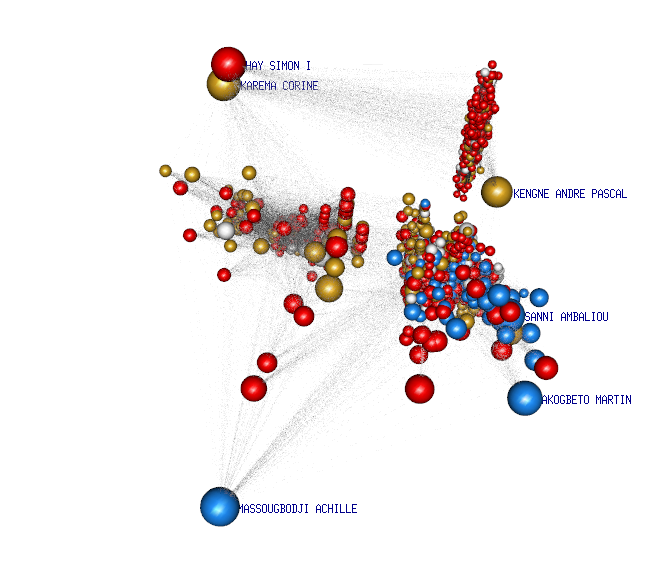
\includegraphics[scale=0.3,trim={5cm 0 0 0}]{Chapters/malaria/statMod/lnm_mod5_nodes.png}
\vspace{2px}\\
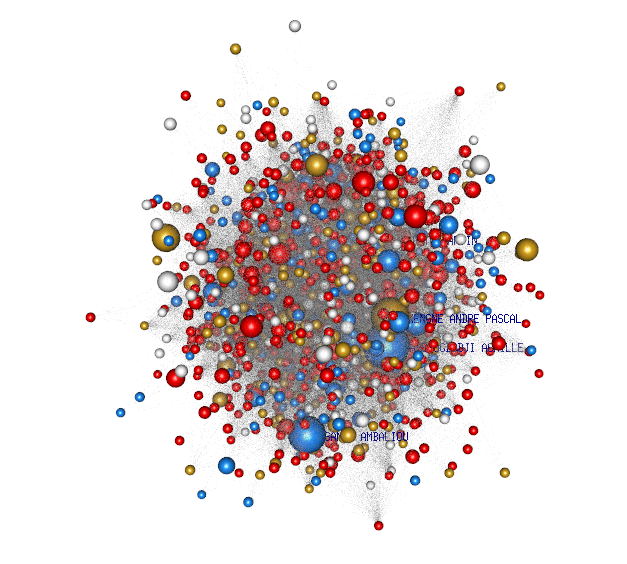
\includegraphics[scale=0.3]{Chapters/malaria/statMod/lnm_mod6_all.png}
\caption{Visualizations of the Malaria co-authorship network with layouts determined according to the inferred latent eigenvectors in the LNM models (International (Red); Regional (Gold); Local (Blue)).
% with no pair-specific covariates (top), nodal covariates (middle), and all covariates (bottom).
}
\label{fig:malaria_lnm_viz}
\end{figure}

The ROC curves on figure \ref{fig:malaria_lnm_roc} show that the first two models appear to be comparable in their performance from the perspective of edge status prediction with an Area Under the Curve (AUC) being roughly 98.8\%. %The third model, with added dyadic covariates, has a perfect fit to the observed network data.

\begin{figure}[!h]
\centering
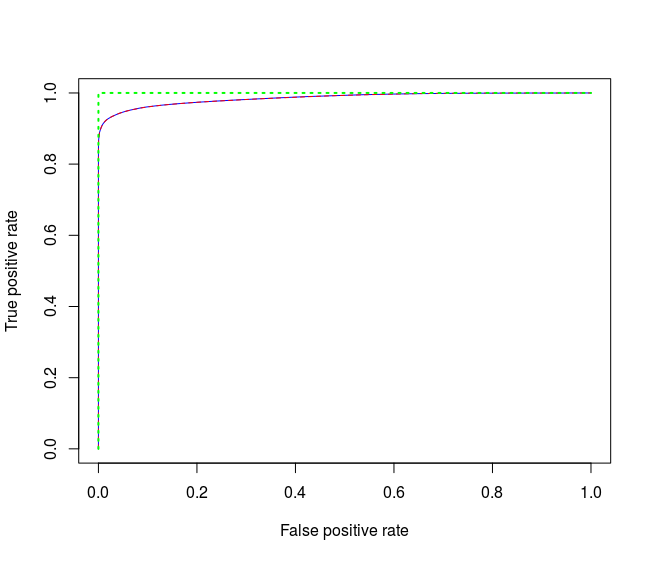
\includegraphics[scale=0.75]{Chapters/malaria/statMod/lnm_ROC.png}
\caption{ROC curves comparing the goodness-of fit of the Malaria co-authorship network for three different eigenmodels, specifying (i) no pair specific covariates (blue), (ii) nodal covariates (red), and (iii) nodal and dyadic covariates (green), respectively.}
\label{fig:malaria_lnm_roc}
\end{figure}
~\\
\pagebreak
\section{Discussion and Conclusion}
\label{sec:malaria_discussion}
In this chapter, we provide insights in the structural characteristics of the malaria co-authorship network in the Republic of Benin over a relatively long period. The 20 years of data collected coincides with the onset of active malaria research from 1996 until today. The significant increase in malaria research and collaborations (figure \ref{fig:malaria_dist}) between the authors over the years is an expected finding given the regain and renewed interest in malaria control and elimination goals set forth \cite{alonso_research_2011, breman_eradicating_2009}. Our results show that the mechanism underlying the formation of the malaria co-authorship network in Benin is not random. It further demonstrates that the malaria research collaboration network in Benin is a complex network that seems to display small-world properties (often referred to as "six degrees of separation"). \\%~\\
The non-trivial number of authors with higher order of magnitudes confirms the presence of closed research groups where collaborative research likely happens only among members. In other words, interdisciplinary collaboration tends to occur at higher levels between prolific researchers with the majority of the collaborations happening between researchers from the same scientific communities. Prominent authors with long tenure tend to collaborate with similar authors, young or less prolific authors tend to collaborate with both prolific authors and authors with very few collaborations. Similar findings were reported by Janet Okamoto \cite{the_centers_for_population_health_and_health_disparities_evaluation_working_group_scientific_2015} who studied scientific collaboration on a much smaller scale. %\\
Key brokers facilitate scientific collaborations within and outside their scientific community \cite{bellanca_measuring_2009}. Betweenness centrality measures identify such brokers who are important hubs for inter and transdisciplinary research. Many of the main brokers proved to also be the most connected and the most central authors confirming the presence of long publishing tenure authors in our network \cite{li_co-authorship_2013}. %\\
The flow of information in this network in Benin is slow as it only relies on 16 authors representing less than 1\% of all the authors in the network. Such a low information flow was also reported by Salamatia and Soheili \cite{salamati_social_2016} in a 2016 study on a co-authorship analysis of Iranian researchers in the field of violence. Generally, the most important authors in a co-authorship network are the ones with the highest degree of collaborations \cite{bales_social_2008, bales_evolution_2011}. However, to the long-term substainability of the malaria research network in Benin, the 16 authors identified as cut vertices are the most important authors. In other words, the removal of less than 1\% of the authors from the network would lead to its collapse. Such a collapse would undoubtedly be detrimental to the future of malaria research in Benin. This finding clearly confirms the conclusion of Toivanen and Ponomariov \cite{toivanen_african_2011} that the African research collaboration network is vulnerable to structural weaknesses and uneven integration.\\%~\\
Small-world networks are known to have small shortest path distance and a high clustering coefficient. Although this co-authorship network seems to display such properties, the Monte-Carlo simulations revealed that the observed network has unexpected properties compared to classic small-world networks. A study of co-authorship network conducted on Chagas disease has found similar findings \cite{gonzalez-alcaide_scientific_2012}. Unlike our study, the authors of the Chagas disease co-authorship study did not deepen their analysis to confirm the small-world nature of their observed network. Other mechanisms such as preferential attachment have been found to explain the structure of international scientific collaboration network \cite{wagner_network_2005}. Unlike those studies, our network displayed unexpected properties that are more extreme than the 4 mathematical models we simulated. Our network has significantly higher clustering than expected from the 4 mathematical models presented here. One observation we are sure of is that none of the random graph models used here tend to explain the growth and the structure of the malaria co-authorship network in Benin. We therefore claim without any doubt that the structure and growth of our network is not random confirming the presence of hidden factors explaining the current structure of the network. Assessing such factors and the extent to which they influence scientific collaborations is important for the future of malaria research and its long-term sustainability. Unfortunately, none of the proposed mathematical models seem to accurately describe the observed structure of the network. To address these limitations, advanced statistical modeling was used to further explain the structure of the network. \\%~\\
Our first approach to modeling our network relied on the use of SBM. In addition of being a model based clustering method, the SBM identified important organizational and interactional patterns in the network. It identified a large clique of mainly international researchers with little or no collaborations with other research groups.
%%%Added from suggested corrections
It also identified the main broker authors in the network. For example, in the first two visualizations on figure \ref{fig:malaria_lnm_viz}, the brokers with affiliations to national institutions are MASSOUGBODJI ACHILLE, AKOGBETO MARTIN, and SANNI AMBALIOU. These authors are also the ones with the highest citation counts. Such an observation is not surprising given their long tenure, their publication records, and known expertise in malariology, parasitology and medical entomology. 
%%%
The overwelming dominance of regional and international players in the network is consistent with previous observations by Onyancha and Maluleka \cite{onyancha_knowledge_2011} who concluded on a much higher likelihood of Sub-Saharan African countries to collaborate with non-African states. \\
Overall, the ERGM and TERGM show that the mechanistic phenomenon driving collaboration ties in the malaria research in Benin is influenced by homophily on the type of affiliation (national, international or regional) and on membership to a research group or cluster, verifying therefore our third hypothesis. The models clearly show that the dominance of the Beninese malaria research arena by international and regional players, and further demonstrates the lower likelihood of local Beninese researchers to establish international collaboration ties compared to regional researchers. This latter finding has been confirmed by the LNM which also confirms our second hypothesis. The ERGM and the TERGM revealed that factors such as number of publications, number of citations and number of collaborations are associated to higher likelihood to establishing collaboration ties, confirming therefore our first hypothesis. \\
It is worth noting that many of the studies on co-authorship network analysis are descriptive in nature. This study is one of the rare co-authorship network analysis to model a co-authorship network using advanced statistical models. ERGM is the leading approach to modeling network \cite{schmid_exponential_2017}. The literature has reported application of this model in studying various social network such as the analysis of friendship and obesity \cite{valente_adolescent_2009,de_la_haye_obesity-related_2010}, the exploration of the association between hormone and social network structure \cite{kornienko_hormones_2014}. Similarly to friendship networks, the use of ERGM to model co-authorship networks is easily justified. However, the size of our network prevented the fitting of complex models including dyadic and structural terms. In addition, our best ERGM model failed to adequately fit the observed network data. This lack of goodness-of fit, according to Hunter, Goudreau and Handcock \cite{hunter_goodness_2008}, could be improved by including the geometrically weighted edgewise shared partner, geometrically weighted dyadic shared partner, and geometrically weighted degree network statistics to our model. Although, we follow such recommendations by including these structural network statistics to our final model, the ERGM model failed to converge after a maximum of 1,000 iterations. At about 750 iterations, we noticed that the processing became both computationally intensive and expensive in terms of CPU time and memory usage. In a recently published paper, Schmid and Desmarais \cite{schmid_exponential_2017} acknowledged the difficulty of fitting network which size is of the order 1,000 vertices using ERGM. They recommended that using the maximum pseudolikelihood estimation (MPLE) instead of the Monte Carlo maximum likelihood (MCMLE) could tremendously reduce computation time. Having followed these recommendations too, the ERGM model containing dyadic and structural terms still failed to converge. By finally including temporal dependencies and fitting a temporal ERGM, we have tremendously improved the fitness with a predictive performance of roughly 80\%. Nevertheless, we suspect that the number of edges, the large size of the network added to the possibility of hidden/latent variables might justify the failure of the models containing the dyadic and structural endogenous terms to converge. We remedy this situation by applying LNM to the observed network data. \\
All three latent network models (LNM) proved to be successful in fitting the observed network data. 
%The fact that the third latent network model include all nodal and dyadic variables could explain its perfect fit. In addition, there was less structure left to be captured by the latent variables in this model. On the other hand, the first two latent network models gave us confident in validating the results of the TERGM. \\
A study by Kronegger et al. \cite{kronegger_collaboration_2012} conducted an investigation aiming at describing the collaboration in Slovenian scientific communities using data from four different disciplines. Their methodological approach is consistent with ours. The main difference is their application of Stochastic Actor-Oriented Model (SAOM) on the dynamics of their co-authorship networks. Since the SAOM is an actor-oriented modeling method and we are interesting in tie prediction here, we relied rather on a tie-oriented approach by applying the TERGM to our network data. \\
Our results suggest that the regain in Malaria research funding has appealed to research groups all around the world, hence the explosion in publications number and research collaborations. 
As the disease continues to be main public health concern in the Republic of Benin, it is essential to consolidate the knowledge generated from the numerous studies on the disease and reinforce the different  communities involved in the research effort. In addition, there is an urgent need to reinforce the malaria research network in Benin by continuously supporting, stabilizing the identified key brokers and most productive authors, and promoting the junior scientists in the field. However, we observed a tendency of the international researchers to only collaborate among themselves. Although the rise in scientific collaboration between advanced and developing nations \cite{wagner_science_2001}, the latter observation may limit effective and sustainable technology transfer in Benin. It is possible that some of the isolated cliques within the network have top-notch research capabilities and skills researchers affiliated to Beninese institutions can acquire, should the research groups be more inclusive. Unfortunately, our visualizations showed that broker authors that liaison those closed groups to national researchers tend to be regional or international researchers as well. We therefore recommend, that policies should be designed, at international, regional and country level, to diversify research groups operating in any Sub-Saharan African countries. Such policies will ultimately enable effective technology transfer, multidisciplinarity, and promote junior African researchers to advance the search of a solution to the Malaria problem in Africa and particularly, in Benin.


%%%%%%%%%%%%%%THIS SECTION IN GENERAL CONCLUSION
%Since co-authorship networks are dynamic in nature, the application of temporal or dynamic modeling techniques is the major strength of our research. Other strengths include its application of not only descriptive methods but also robust network analysis methods such as inferential methods like Monte-Carlo simulations, unlike most studies on co-authorship analysis. Our data mining strategy involved a robust machine learning algorithm that helped address the crucial issue of the disambiguation of authors names and assign a unique identification to each of them. This technique maintained a good quality of the data collected throughout the pre-processing and analysis steps. To the best of our knowledge, our study is the first to describe the malaria research collaborations network via co-authorship network analysis in Benin. It is also the first to apply statistical network models to investigate co-authorship network in a specific research area in an African country.\\%~\\
%The fact that our study collected data only from the Web Of Science can be considered as an important limitation of this study. However, according to Falagas and colleagues \cite{falagas_comparison_2007}, who compared PubMed, Scopus, Web Of Science and Google Scholar in their paper, the Web Of Science appears as a reasonable scientific database source for our analysis. In addition, it proved to cover a wide range of both old and recently published papers. Falagas and colleagues \cite{falagas_comparison_2007} found PubMed to be the optimal choice in terms of scientific database. For that reason we did run the same bibliographic search in PubMed. Unfortunately, the Web Of Science returns more relevant data than PubMed. Another limitation worth noting is that this study only looks at a snapshot of the malaria research network on a static fashion. There is also a need to apply dynamic statistical models such as Temporal Exponential Random Graph \cite{leifeld_temporal_2015} and Dynamic Stochastic Block \cite{matias_statistical_2016} modeling to better understand the temporal dynamic of collaboration formation in this network. Yet another limitation is inherent to the nature of all co-authorship studies. Collaborators, in a co-authorship network, do not often come from the same scientific discipline, or do not play the same roles on a particular research project. The data we collected did not allow us to accurately assess or even infer the disciplines each author came from or their specific contribution in the published document.\\%~\\
